\chapter{Implementation}

Differential GPS was evaluated as a suitable method to enhance the GPS position accuracy to the required level of 1 meter RMS.
This chapter documents the proccess of implementing it as a proof of concept.
Although this project is not planned to be used in this years competition, the system is designed to work with the current hardware of project TELL.
Section \ref{sec:tell_infrastructure} shows what is already implemented in project TELL.
How DGPS can be integrated into this infrastructure is explained from section \ref{sec:system_overview} onward.

\section{TELL Organization and Infrastructure}\label{sec:tell_infrastructure}

At the time of writing, the rocket of prject TELL is being made ready to ship to the U.S. for the 2018 Spaceport America Cup.
The whole project is divided into the 7 subteams: Simulations, Structures, Propulsion, Avionics, Control, and Recovery.
This bacelor thesis is a project of the Avionics subteam.
The Avionics subteam is responsible for the sensor data aquisition which used by the controll and for logging, as well as a telemetry link to a ground station to transmit the most important metrics to monitor the flight performance and recover the rocket.
Apart from the rocket called TELL \rom{1}, the hardware consists of a ground station with laptop, telemetry link, and GPS reference station.

\subsection{The Rocket}

TELL \rom{1} is the vehicle that shall propel the 4 kg payload to the target apogee of 10'000 feet (3048 meters) at the competition.
In figure \ref{fig:tell_1} it is shown in the wind tunnel test.
It has a length of 2.42 meters, weights 24 kg at liftoff, and is porpelled by a solid motor with an average thrust of 2245 N.
With those parameters, the rocket is designed to overshoot the target apogee.
Air brakes driven by a controll loop are used to correct the apogee.

\begin{figure}[ht]
 \centering
 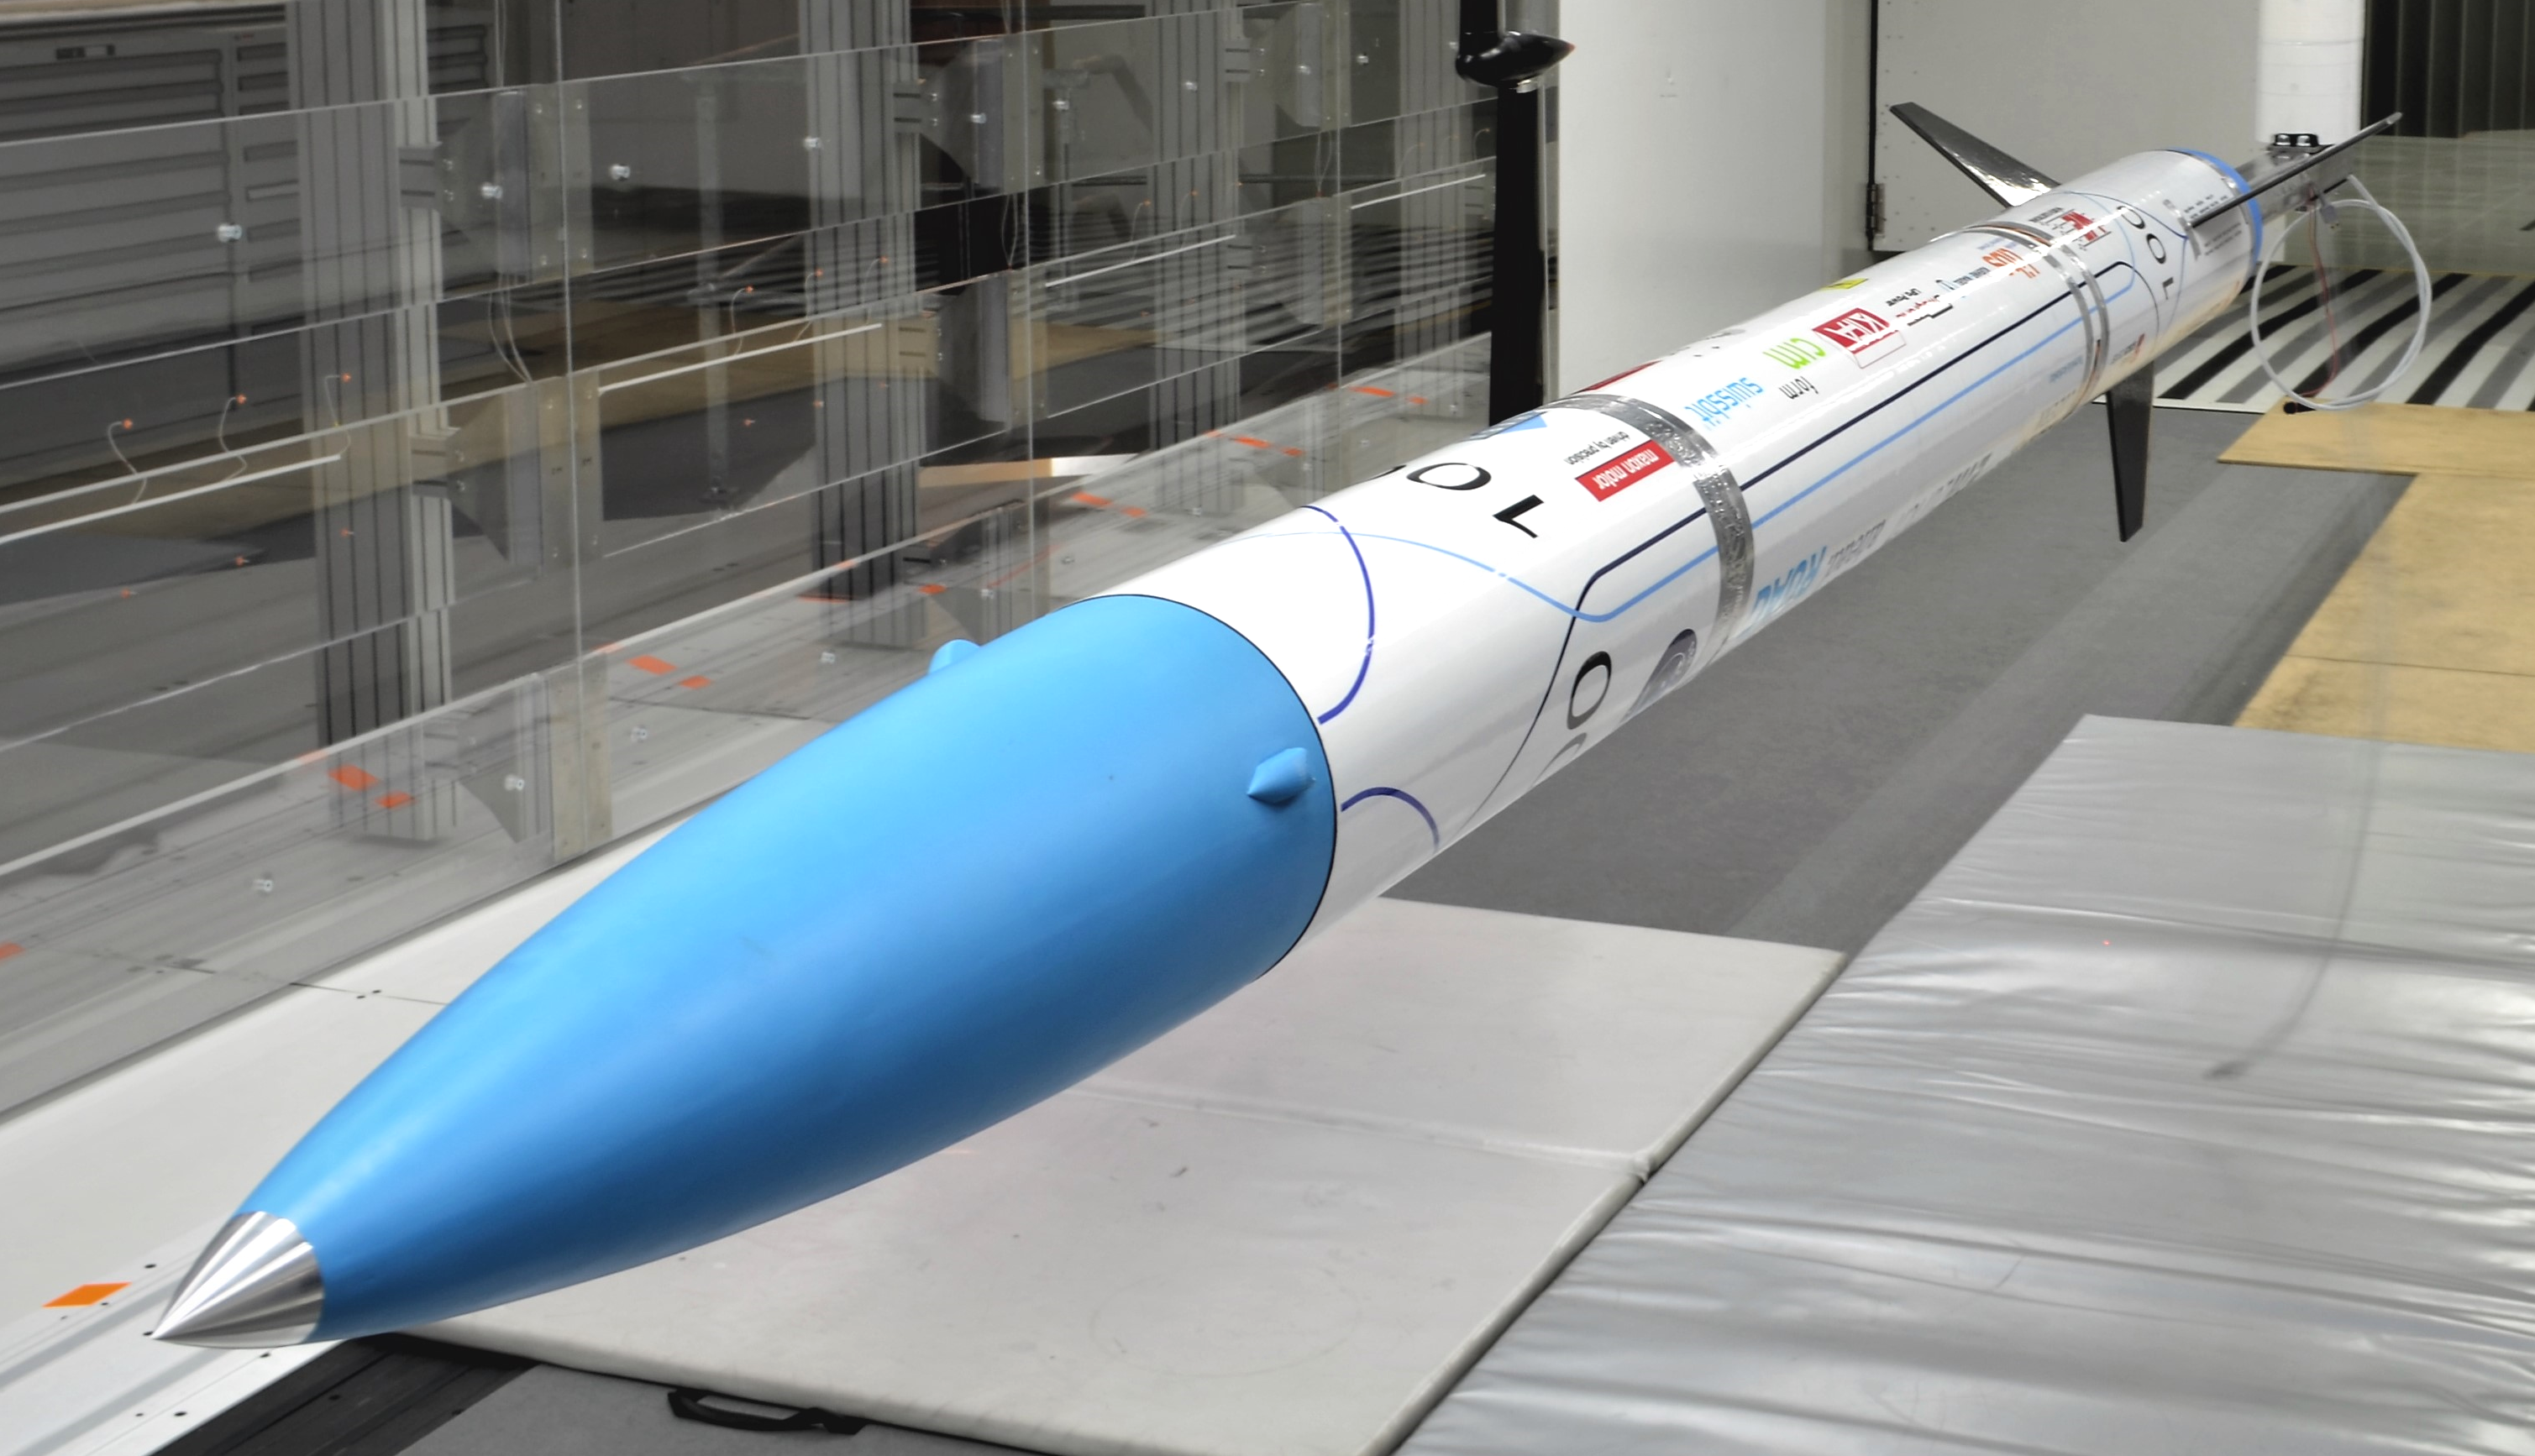
\includegraphics[height=6cm]{images/TELL_1.png}
 \caption{TELL \rom{1} in the wind tunnel}
 \label{fig:tell_1}
\end{figure}

The avionics on the rocket are split into the two parts nasecone avionics and lower body avionics as shown in figure \ref{fig:tell_structure}.
Both parts are the same appart from the GPS and telemetry in the nosecone, and two additional barometers, rocket motor temperature sensor and payload interface for the lower body avionics.
Sensors that both parts have separately are an acceleromert, magnetometer, gyroscope and climate sensor.
Both parts also log their collected data to a seperate SD card.
This is done to have redundancy and to be able to have sensors in all parts of the rocket.
The two parts are connected over a wireless link to be able to communicate after the nosecone is popend off at the first recovery event.
The central component of each avionics module is an ARM M4 microcontroller that acts as the flight controller.
It connects to all the sensors and communication modules of its half of the rocket.

The nosecone avionics has two GPS antennas with a separate receiver for each.
One is directed upwards to have reception in the time from launch to the apogee.
The other is directed downwards to have reception after the nosecone is hanging upside down after the first recovery event.
The telemetry transmitter and antenna are also implemented in the nosecone.
As the transmitter, the XBee-PRO SX module is used.
It transmitts on the frequency band from 902 to 928 MHz, which is open for public use in north america, where the competition is taking place.
With a transmitting power of 1 W, it can establish a link over a range of up to 105 km.

\begin{figure}[ht]
 \centering
 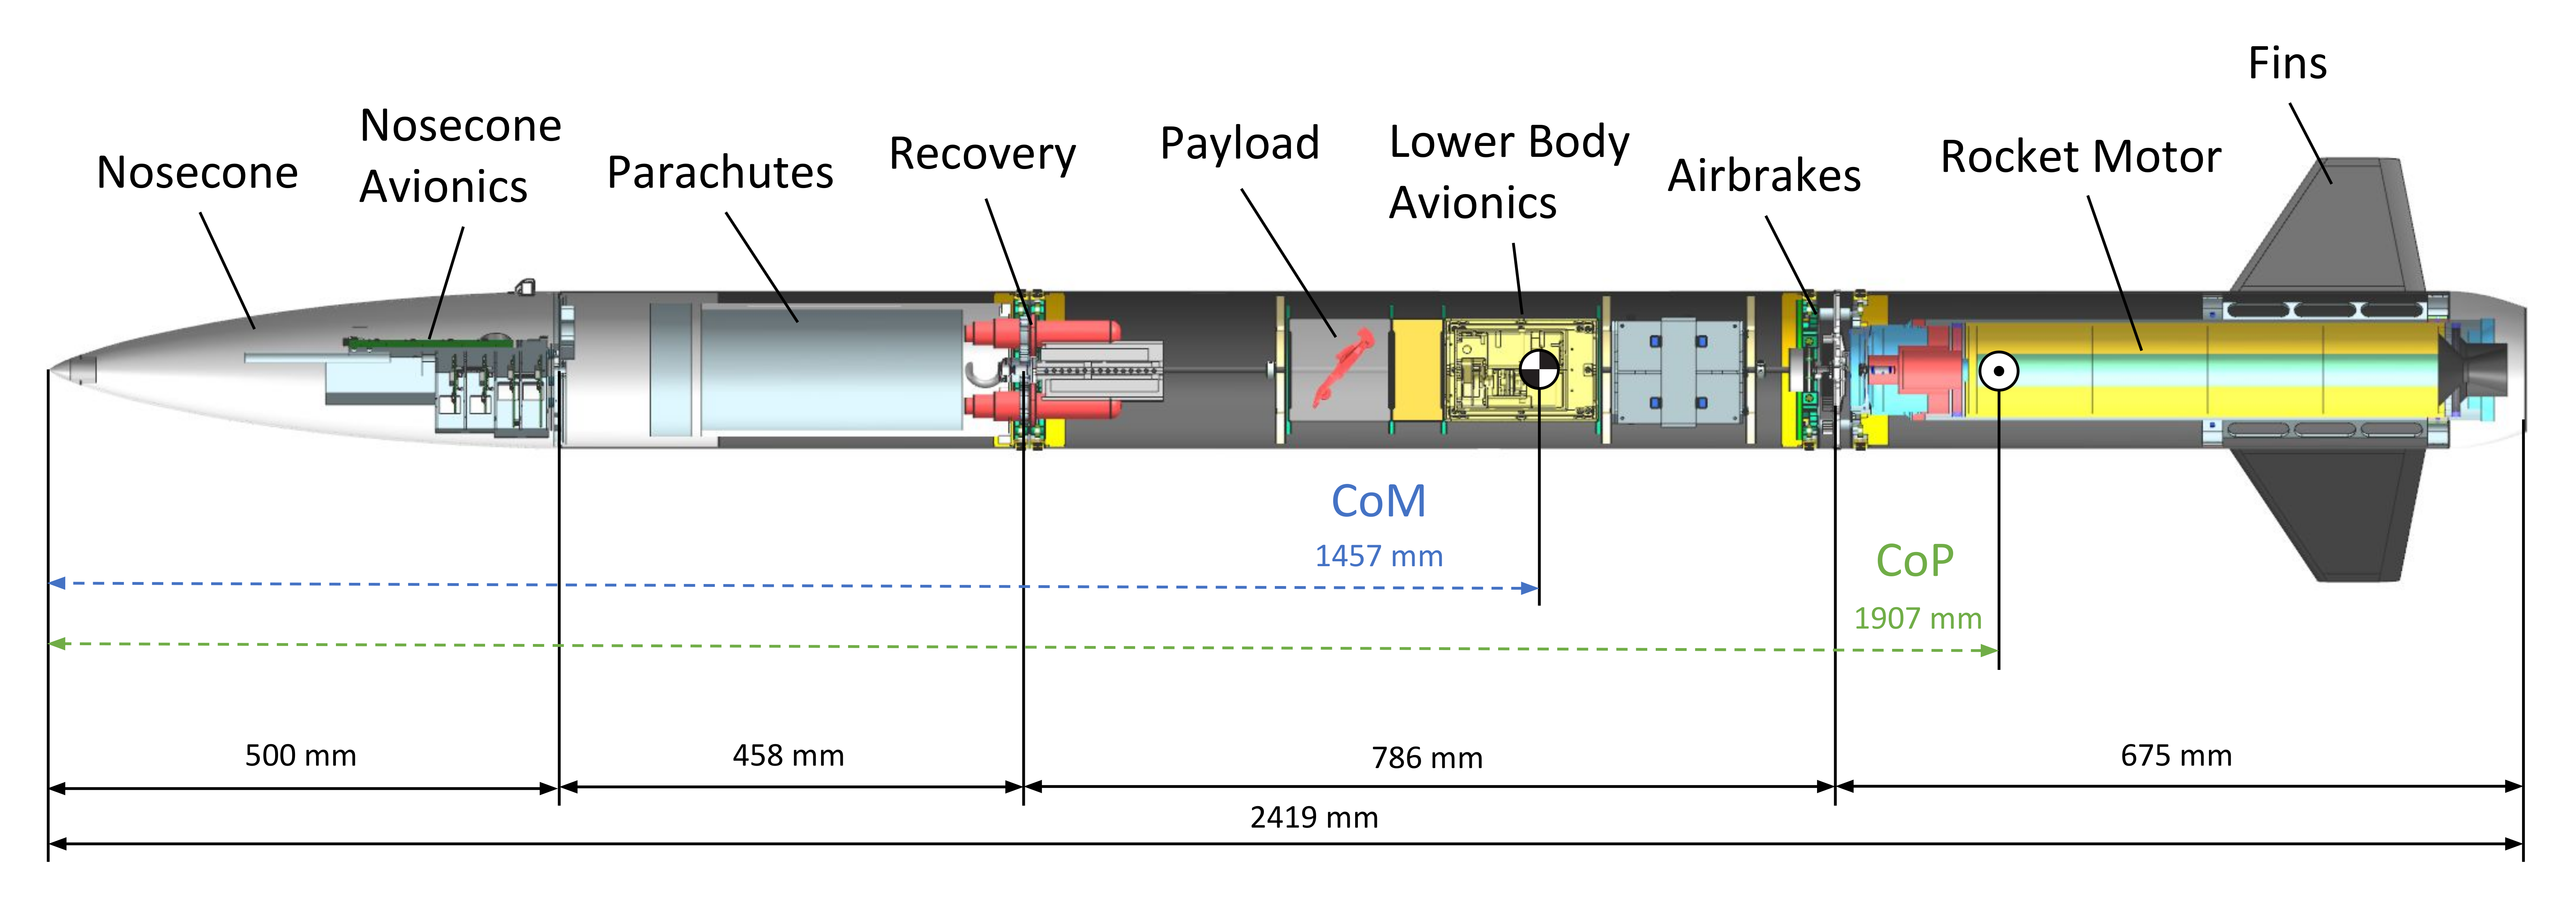
\includegraphics[width=\textwidth]{images/TELL_Structure.png}
 \caption{Overview of TELL}
 \label{fig:tell_structure}
\end{figure}

\subsection{The Ground Station}

The central part of the ground station is the a laptop that displays the live flight metrics.
Connected to it over USB is a second XBee module, that receives the telemetry data sent by the rocket.
A directional antenna is used to receive the downstream.

In this years project, it is planned to do post-processing DGPS to analize the trajectory.
GPS raw data has to be logged on the rocket and at a reference station in order to do that.
For post-processing DGPS, no data link is needed to the rocket.
A GPS receiver is placed at the ground station to act as the reference station.
The GPS module M8T fron u-blox was choosen for this purpose and is used in the rockets nosecone avionics, as well as at the ground station.
The speciality of the M8T module is, that it provides raw GPS data like the measured pseudoranges.
This is needed for post-processing DGPS.

\section{System Overview}\label{sec:system_overview}

The difference of the DGPS system described in this thesis to the post-processing one used by project TELL is when the corrected position is availabel.
A real-time system is needed that the corrected position can be directly used to controll the rocket.
This adds the requirement for a live PRC calculation, a data link to the rocket, and the inclusion of the corrections into the position estimation on the rocket.

Let's start with the data link.
Is is needed to send the corrections from the reference station, which is in this case the ground station, to the rocket.
With the telemetry system, a link is already established.
Although this is only a downlink for project TELL, the used XBee modules can be configured for a two way communication link.

For the DGPS to work, the measured pseudoranges on the rocket have to be corrected with the PRCs before they are used to estimate the position.
There are two possible ways to achieve this.
For the first way, the receiver would have to provide raw GPS data to the flight computer where the PRC can be added.
The position would then have to be estimated outside the receiver by the flight computer.
The challenge with this approach is, that the implementation of a position estimation algorithm from raw GPS data is huge development effort, especially on a microcontroller.
The second way is to choose a GPS receiver that accepts PRCs in a certain format and includes them in its position estimation.
This method has the advantage of a much smaller development effort because the position estimation can be left to the receiver.
The drawback is that the specific DGPS protocol accepted by the receiver has to be used, which limits the design freedom.
Both methos are possible with the current M8T GPS receiver.
It was specifically choosen because it outputs raw GPS data like the pseudoranges.
It also accepts PRCs in the form of a RTCM data stream, which is described in setion \ref{sec:rtcm}.
The second approach, where the receiver estimates the position, was choosen for this project to make it feasible to implement the system.
There are other receivers besides the M8T that have this functionality.
The selection of the receiver is addressend in section \ref{sec:receiver}.

Finally, the PRCs have to be generated at the ground station.
A similar trade off between flexibility and small development effort as for the position estimation in the rocket has to be made here.
The PRCs can either be calculated from GPS raw data, or a receiver with integrated reference station functionality can be used.
The decision was made in favor of a custom reference station algorithm.
The development effort is not as big as for a position estimation algorithm.
Also, such a system can more easily be impelemented in parallel to the current post-processing DGPS method, which will always be more precise than a real-time solution for post-flight analysis.
The custom application developed to generate the PRCs is described in section \ref{sec:dgps_message_generator}.

\begin{figure}[ht]
 \centering
 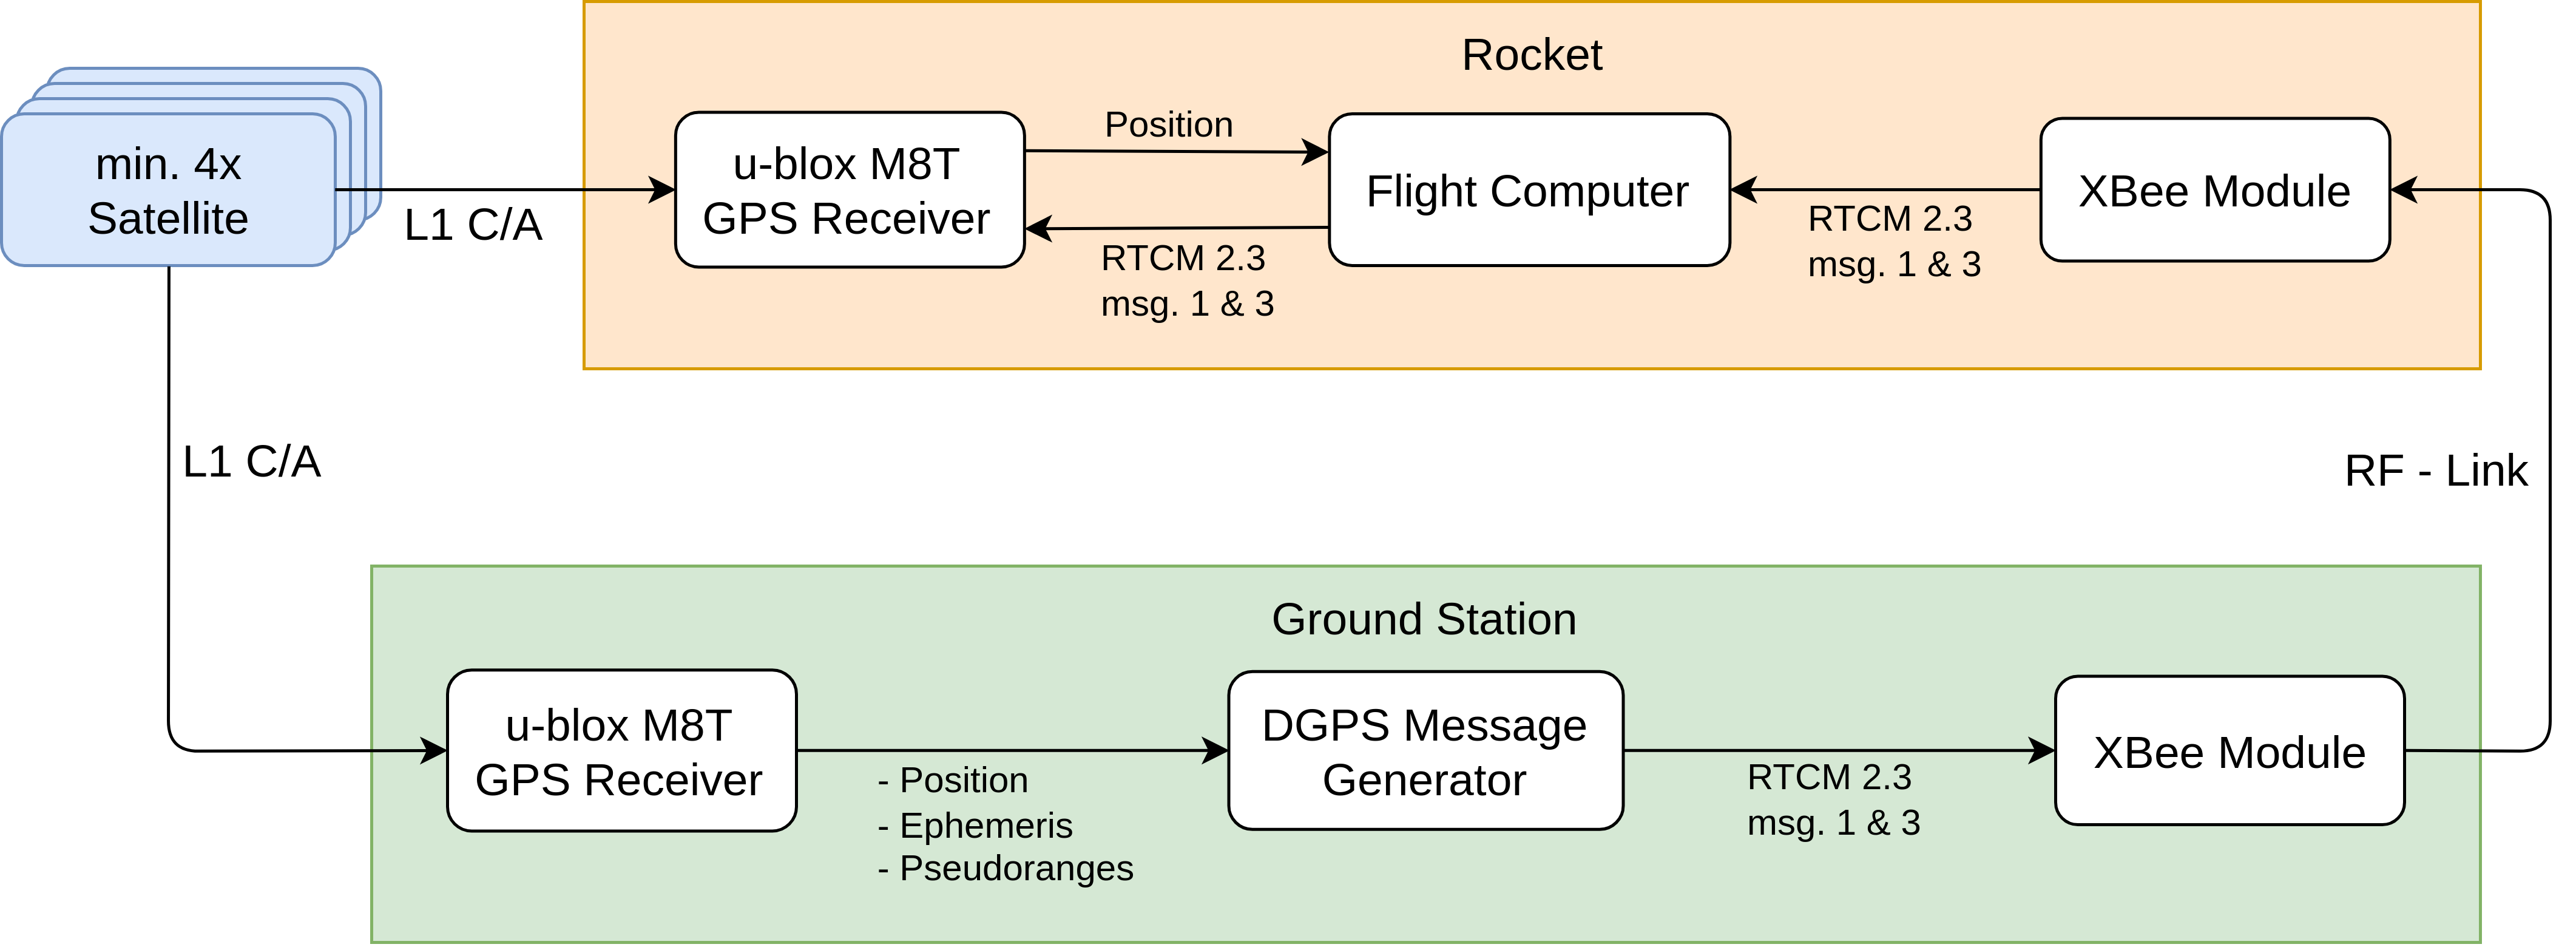
\includegraphics[width=\textwidth]{images/DGPS_System_Overview.png}
 \caption{DPGS data flow}
 \label{fig:data_flow}
\end{figure}

A top level view of the data flow for the planned system is shown in figure \ref{fig:data_flow}.
It starts with the generation of the GPS signals by the satellites.
The standard L1 C/A signals are used.
Both receiver have to receive the signals from a set of at least four satellites for the system to work.
The receiver at the ground station then measures the pseudoranges, decodes the navigation messages, and estimates its position.
It then sends its position, the navigation message bits which include the ephemeris data, and the measured pseudoranges to the ground station laptop over a USB connection.
This data is processed by the custom DGPS message generator application running on the ground station laptop.
The calculated PRCs are packed in messages of the RTCM 2.3 standard.
Message 1 and 3 of the standard are needed by the M8T receiver.
They are sent over another USB connection to the XBee module of the ground station to be transmitted over the RF link to the rocket.
The messages are forwarded to the flight computer in the nosecone, where they are separated from other data and fed into the GPS receiver on the rocket.
This receiver then corrects its pseudoranges with the latest PRCs before estimating the rocket position.

\section{GPS Receiver}\label{sec:receiver}

\begin{minipage}{0.6\textwidth}
  A seen in figure \ref{fig:data_flow}, the M8T receiver used by TELL was also choosen for this project.
  The reasons for this decision were the following:
  \begin{itemize}
  \item output of raw GPS data
  \item support of the RTCM 2.3 standard
  \item same receiver can be used for rocket and reference station
  \item compatibility with post-processing DGPS
  \end{itemize}
\end{minipage}
\hfill
\begin{minipage}{0.37\textwidth}
 \centering
 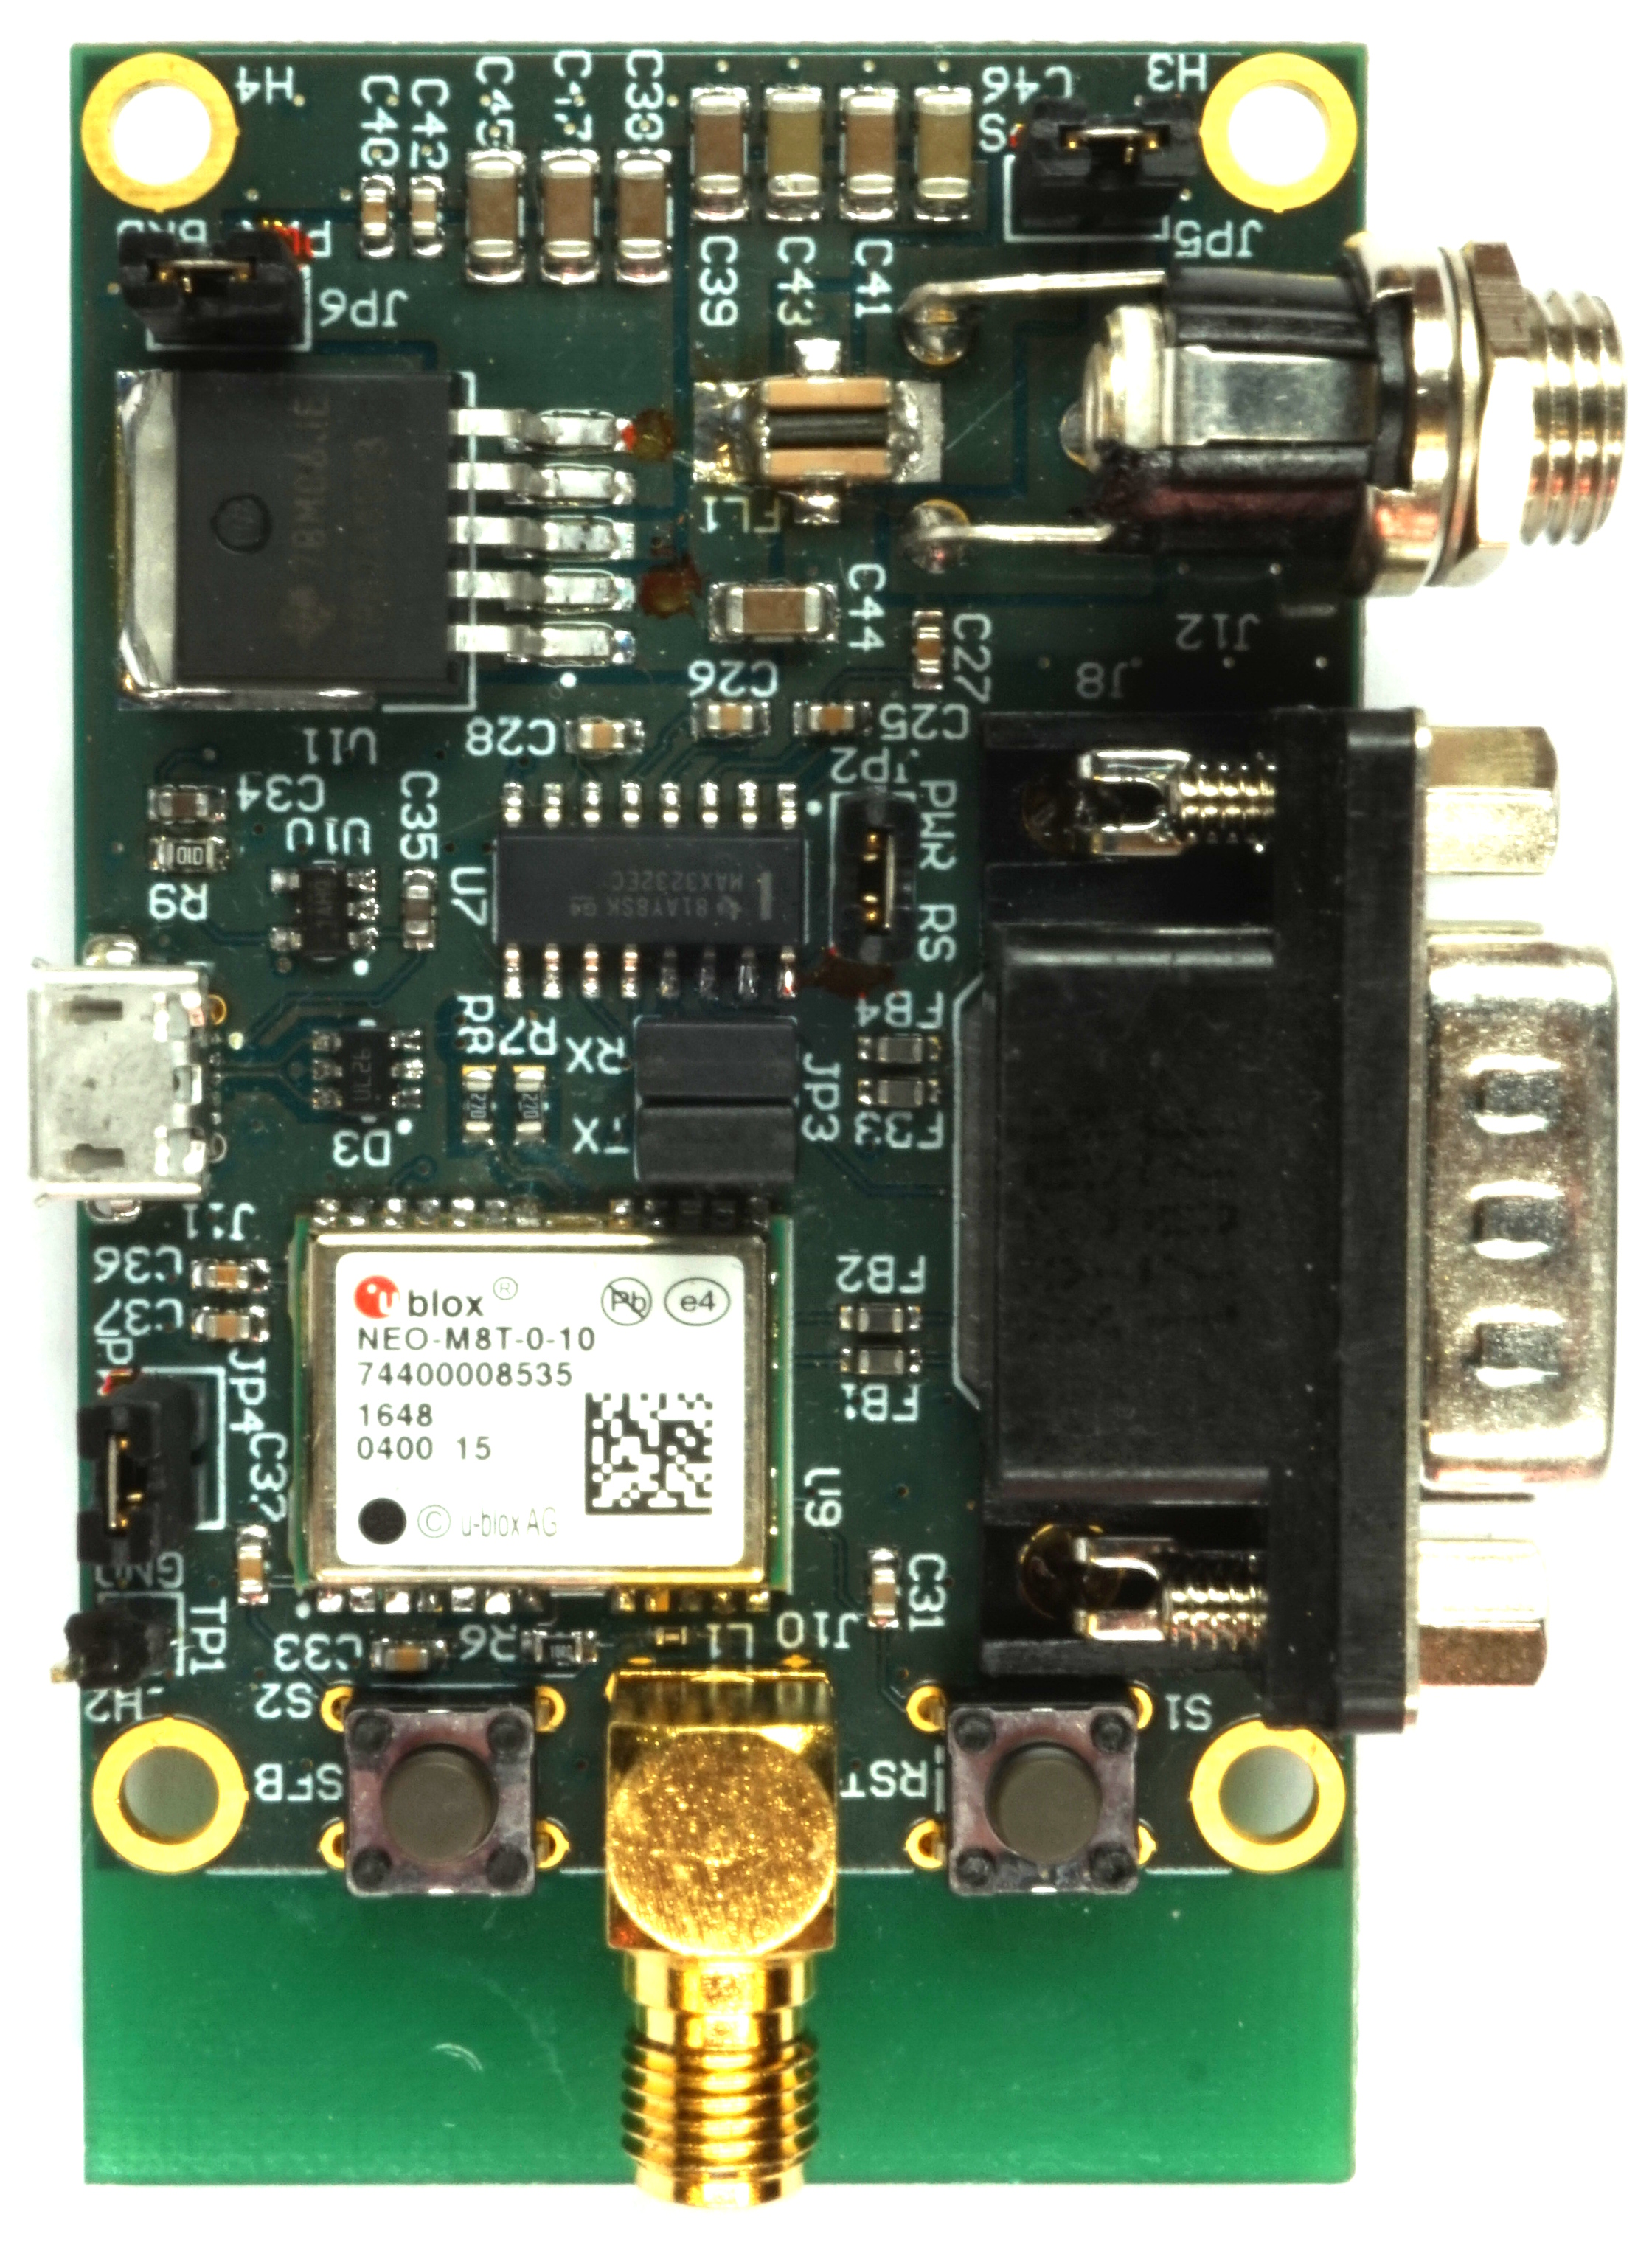
\includegraphics[width=\textwidth]{images/M8T_Receiver_Board.jpg}
 \captionof{figure}{GPS board of project TELL with u-blox M8T receiver}
 \label{fig:m8t_receiver_board}
\end{minipage}

\section{RTCM 2.3 Protocol}\label{sec:rtcm}

\section{DGPS Message Generator}\label{sec:dgps_message_generator}
